\section{Data download and clustering analysis}

Price data on the ETFs is downloaded from Google Finance using the data download functionality built in to the Pandas module for Python.
We use the closing price of the ETF for each day to represent the day's price.
Any ETF with less than 2400 data points is excluded, leaving 93 of the initial 100 ETFs to use for further processing.

To cluster the data, it is necessary to define a distance between assets. We compute the correlation coefficient $C_{ij}$ between the log returns of assets $i$ and $j$, and define the distance between them as
\begin{gather}
d(i,j) = 1 - C_{ij}^2  \in [0, 1].
\end{gather}
This distance will tend to group together assets that are more correlated and/or anti-correlated together.
This is intuitively a reasonable measure, as (1) going long on an asset is the same as going short on an asset that is anti-correlated with it, and we wish to treat short and long assets the same in this analysis, and (2) the difference between a correlation of 1.00 and 0.95 is more significant than between 0.05 and 0.00.

\begin{figure}[tp]
\centering
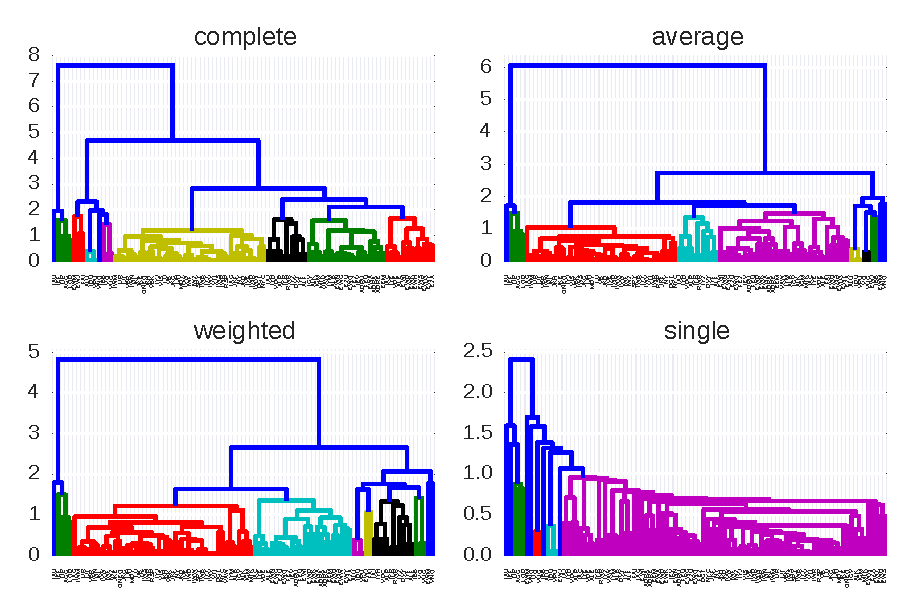
\includegraphics{../pic/dendro_methods.pdf}
\caption{Dendrogram of clusters found by various methods. All non-blue leaves are trimmed by the max-return and the min-std criteria.}
\label{fig:dendrogram}
\end{figure}

To do hierarchical clustering, a method of combining clusters must be defined.
We compare the results of using the various methods built in to the SciPy module for Python: complete, average, weighted and single.
A dendrogram of the clusters found by these methods is shown on Figure~\ref{fig:dendrogram}.
Both the complete, average and weighted methods lead to faily balanced trees.
We choose to use the complete method, as the final clusters found by this method are the most uniform in size.
We choose to use only 15 clusters for the current work, since going to 25 clusters would lead to many single-asset cluster while not breaking up the largest cluster in Figure~\ref{fig:dendrogram} --- an indication that the assets in this cluster are very similar.

\begin{figure}[tp]
\centering
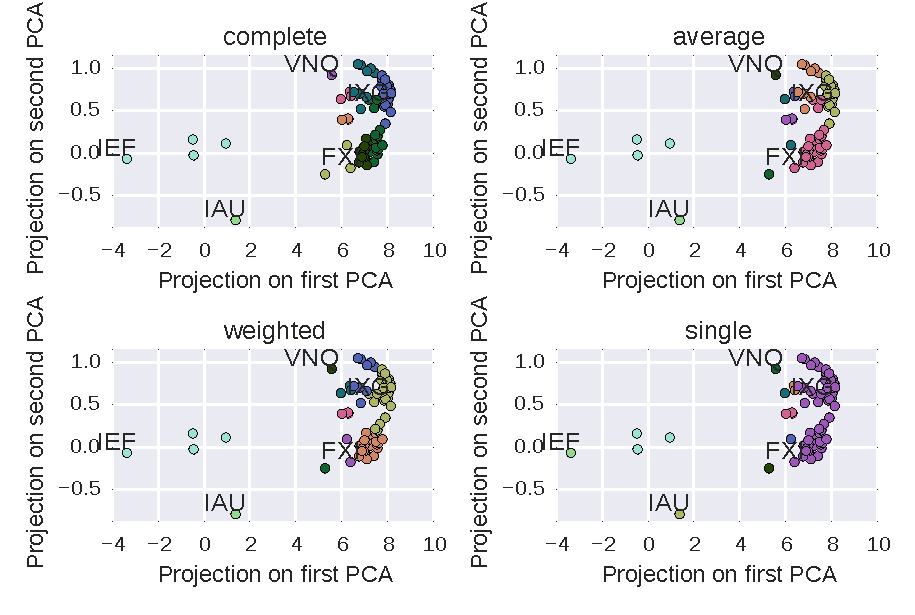
\includegraphics{../pic/pca_methods.pdf}
\caption{Projection of asset correlation onto the largest principal components. These directions account for 78.58\% and 4.51\% of the variance, respectively.}
\label{fig:pca}
\end{figure}

We can further examine the clusters by decomposing $C$ into its principal components $PC_i$, and looking at the projection of the columns of $C$ onto the first two.
This will show a slice of the space defined by $d(i,j)$, and reveal which assets tend to move in a similar manner across the time series.
This slice is shown in fig~\ref{fig:pca}, and clearly shows that 5 assets have radically different behaviour than the others.
In particular, IAU, which tracks the gold price, and IEF, which tracks US treasury bonds, appear to move in a manner inconsistent with the overall market, and are hence clustered differently to these.

\begin{figure}[tp]
\centering
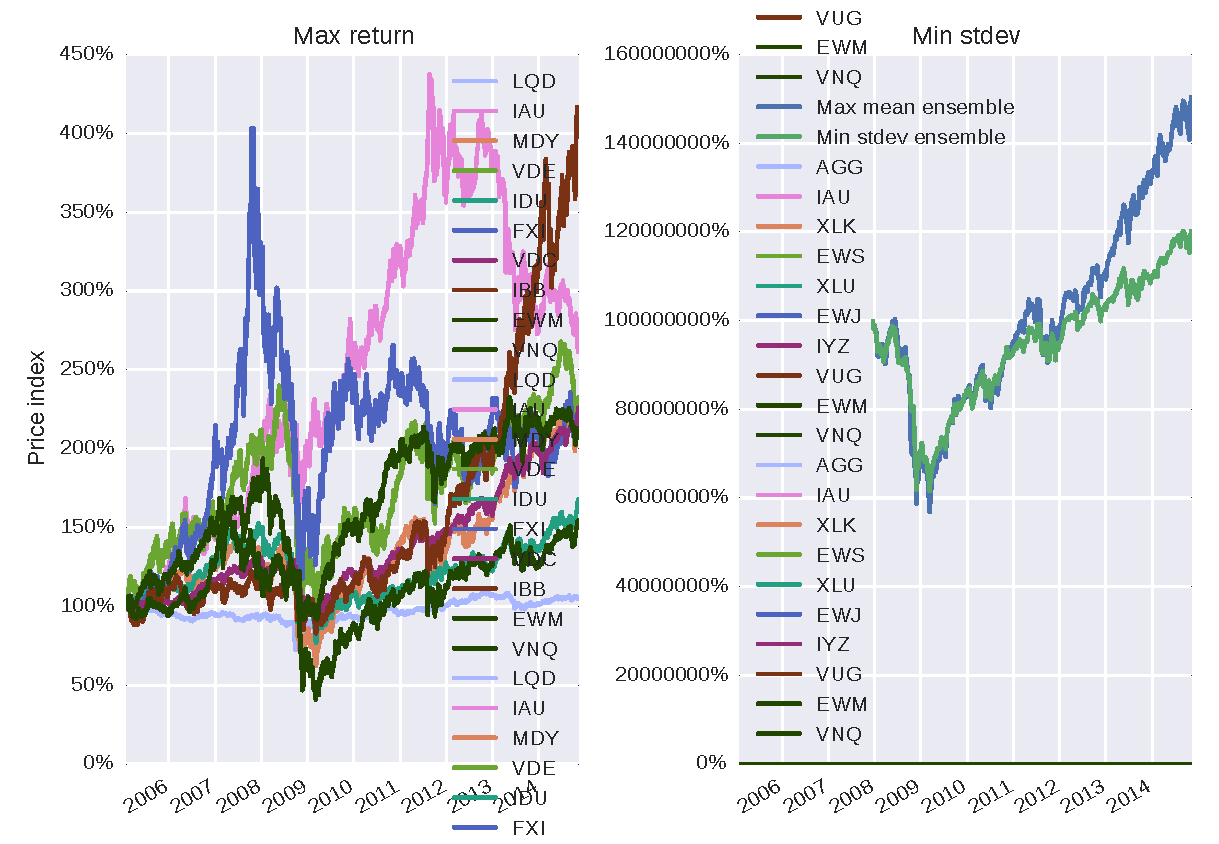
\includegraphics{../pic/prices_selected_assets.pdf}
\caption{Price history for the assets selected by the max-return (top) and the min-stdev criteria (bottom).}
\label{fig:prices_selected}
\end{figure}

In order to prune the tree of assets, we pick from each cluster a single representative asset in two ways.
The max-return criterion picks out the asset which has the highest return across the period, while the min-stdev criterion pick the asset with the smallest standard deviation, i.e.\ the most stable asset.
The assets selected by these two criteria and their associated price histories for the entire period are shown in Figure~\ref{fig:prices_selected}.